%%=============================================================================
%% Graylog
%%=============================================================================

\chapter{Graylog}
\label{ch:graylog}

\section{Installatie en configuratie}

\subsection{Lokale omgeving}
De opzet van Graylog in een lokale omgeving gebeurt relatief eenvoudig. De uitstekende documentatie van Graylog zorgt ervoor dat er meer dan een manier is om dit te doen. De manier waarop hier tewerk is gegaan, gaat als volgt. Er werd een docker-compose.yaml file aangemaakt met de configuratie die te zien is in Listing 6.1. Deze docker-compose definieert drie services, MongoDB, Elasticsearch, en Graylog. MongoDB is verantwoordelijk voor het opslaan van de metadata. Elasticsearch is de database waar alle logs naartoe worden gestuurd. Graylog is de frontend waar de logs zullen getoond worden.

Met het commando `docker-compose up` wordt deze configuratie uitgevoerd en zal de Graylog server samen met Elasticsearch en MongoDb lokaal draaien. Daarna kunnen er logs naar Elasticsearch gestuurd worden. In dit voorbeeld is gekozen voor Fluentd omdat deze een plugin bezit dit GELF als output kan definiëren. GELF werd reeds uitgelegd in ~\ref{subsec:graylog} Graylog. Dit configuratie van Fluentd is te zien in Listing 6.2. Deze configuratie wordt gebruikt bij het uitvoeren van Fluentd in het commando dat te zien is in Listing 6.3.

\begin{lstlisting}[caption=docker-compose.yaml]
   version: '2'
   services:
       # MongoDB: https://hub.docker.com/_/mongo/
       mongodb:
           image: mongo:3
               # Elasticsearch: https://www.elastic.co/guide/en/elasticsearch/reference/6.6/docker.html
           elasticsearch:
               image: docker.elastic.co/elasticsearch/elasticsearch-oss:6.6.1
           environment:
               - http.host=0.0.0.0
               - transport.host=localhost
               - network.host=0.0.0.0
               - "ES_JAVA_OPTS=-Xms512m -Xmx512m"
           ulimits:
           memlock:
           soft: -1
           hard: -1
           mem_limit: 1g
           # Graylog: https://hub.docker.com/r/graylog/graylog/
       graylog:
           image: graylog/graylog:3.0
           environment:
               # CHANGE ME (must be at least 16 characters)!
               - GRAYLOG_PASSWORD_SECRET=somepasswordpepper
               # Password: admin
               - GRAYLOG_ROOT_PASSWORD_SHA2=8c6976e5b5410415bde908bd4dee15dfb167a9c873fc4bb8a81f6f2ab448a918
               - GRAYLOG_HTTP_EXTERNAL_URI=http://127.0.0.1:9000/
           links:
               - mongodb:mongo
               - elasticsearch
           depends_on:
               - mongodb
               - elasticsearch
           ports:
               # Graylog web interface and REST API
               - 9000:9000
               # Syslog TCP
               - 1514:1514
               # Syslog UDP
               - 1514:1514/udp
               # GELF TCP
               - 12201:12201
               # GELF UDP
               - 12201:12201/udp
\end{lstlisting}
\begin{lstlisting}[caption=Fluentd configuratie]
<source>
    @type dummy
    dummy {"info":"message 1"}
    tag dummy 1
</source>

<source>
    @type dummy
    dummy {"warning":"message 2"}
    tag dummy 2
</source>

<source>
    @type dummy
    dummy {"error":"message 3"}
    tag dummy 3
</source>

<match **>
    type gelf
    host 0.0.0.0
    port 12201
    <buffer>
        flush_interval 5s
    </buffer>
</match>
\end{lstlisting}
\begin{lstlisting}[caption=Uitvoeren van Fluentd met configuratie]
$ fluentd -c ./fluent/fluent.conf
\end{lstlisting}

Nadat Graylog en Fluentd volledig zijn uitgerold, kan naar localhost:9000 gesurft worden om de Web Interface te zien. Hier moet eerst nog ingelogd worden met de inloggevens: \begin{itemize}
   \item username: admin
   \item password: admin
\end{itemize}
Na het inloggen kan bij systeem->inputs een databank ingegeven worden waar op zoek wordt gegaan naar logs. Dit scherm is te zien in Figuur 6.3. Hier moet dezelfde poort gebruikt worden als deze gedefinieerd in de docker-compos configuratie van Graylog. Na het toevoegen van een input zijn de verstuurde logs te zien op de startpagina, zie Figuur 6.1. Wanneer extra details van een log gewenst zijn, kan doorgeklikt worden hierop om een detailscherm te verkijgen, zie Figuur 6.2.

\begin{figure}[ht]
    \centering
    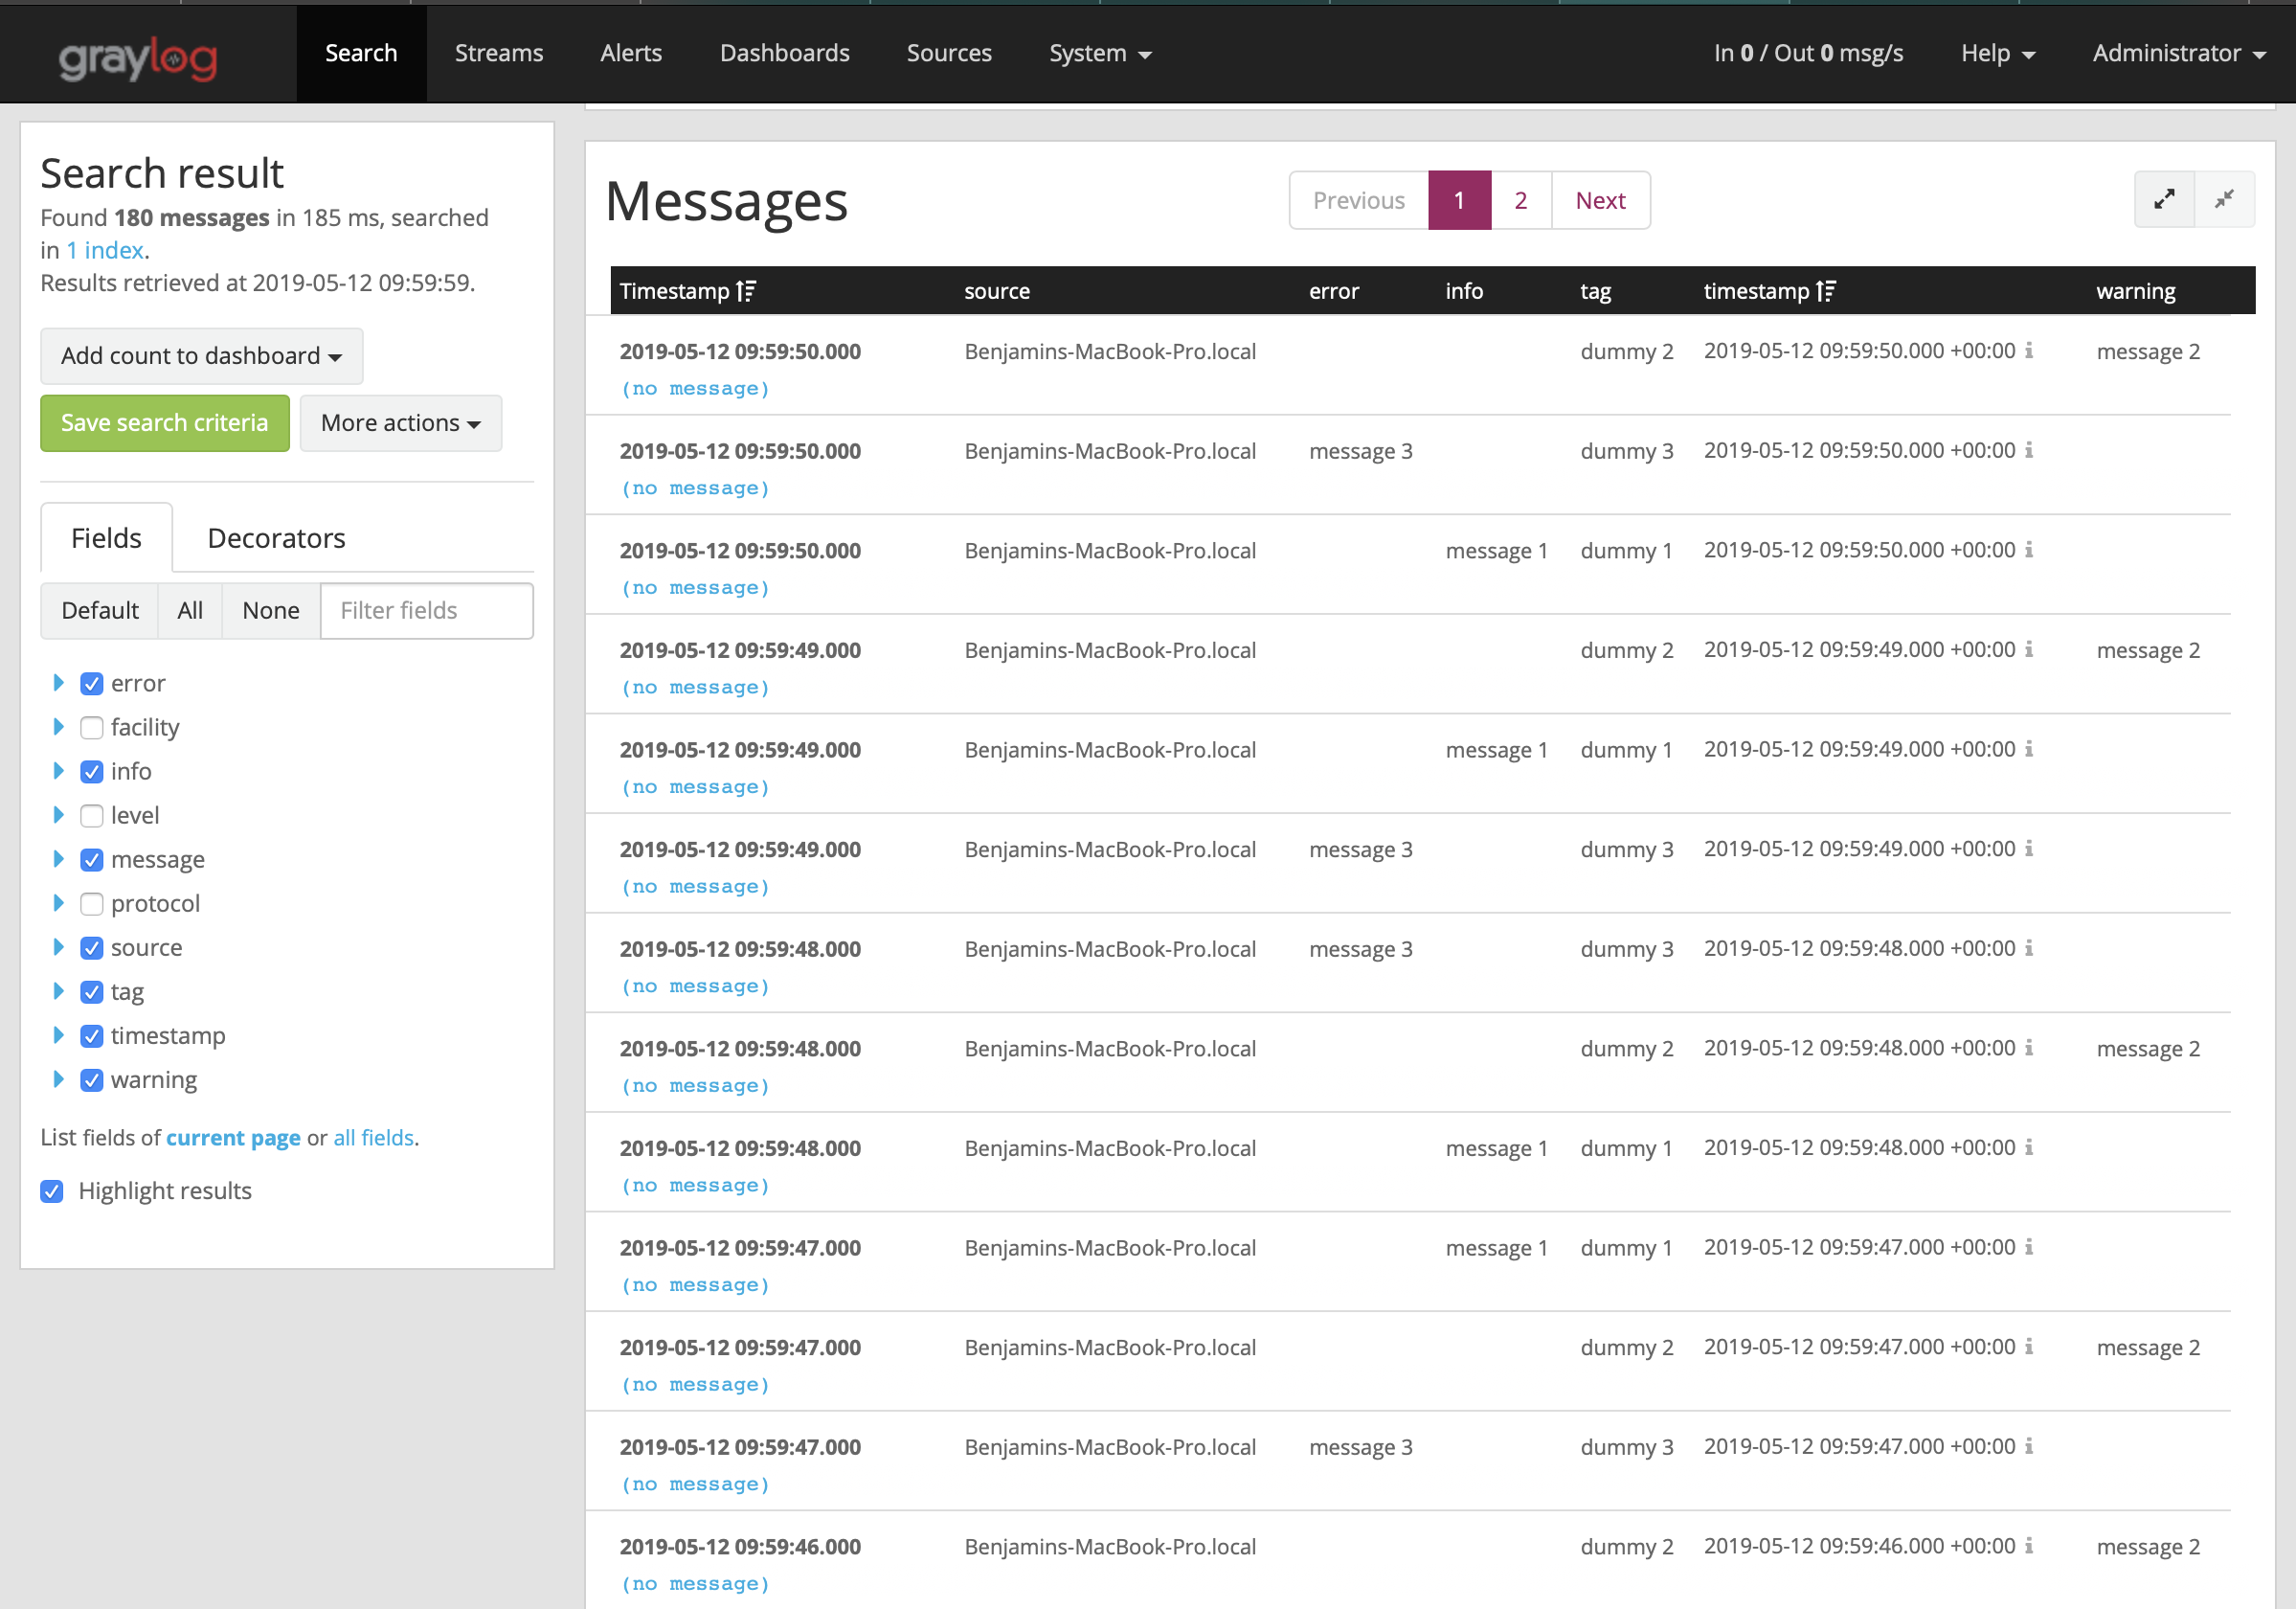
\includegraphics[scale=0.35]{img/graylog_overview}
    \caption[Graylog stack frontend]{Graylog stack frontend}
\end{figure}

\begin{figure}[ht]
    \centering
    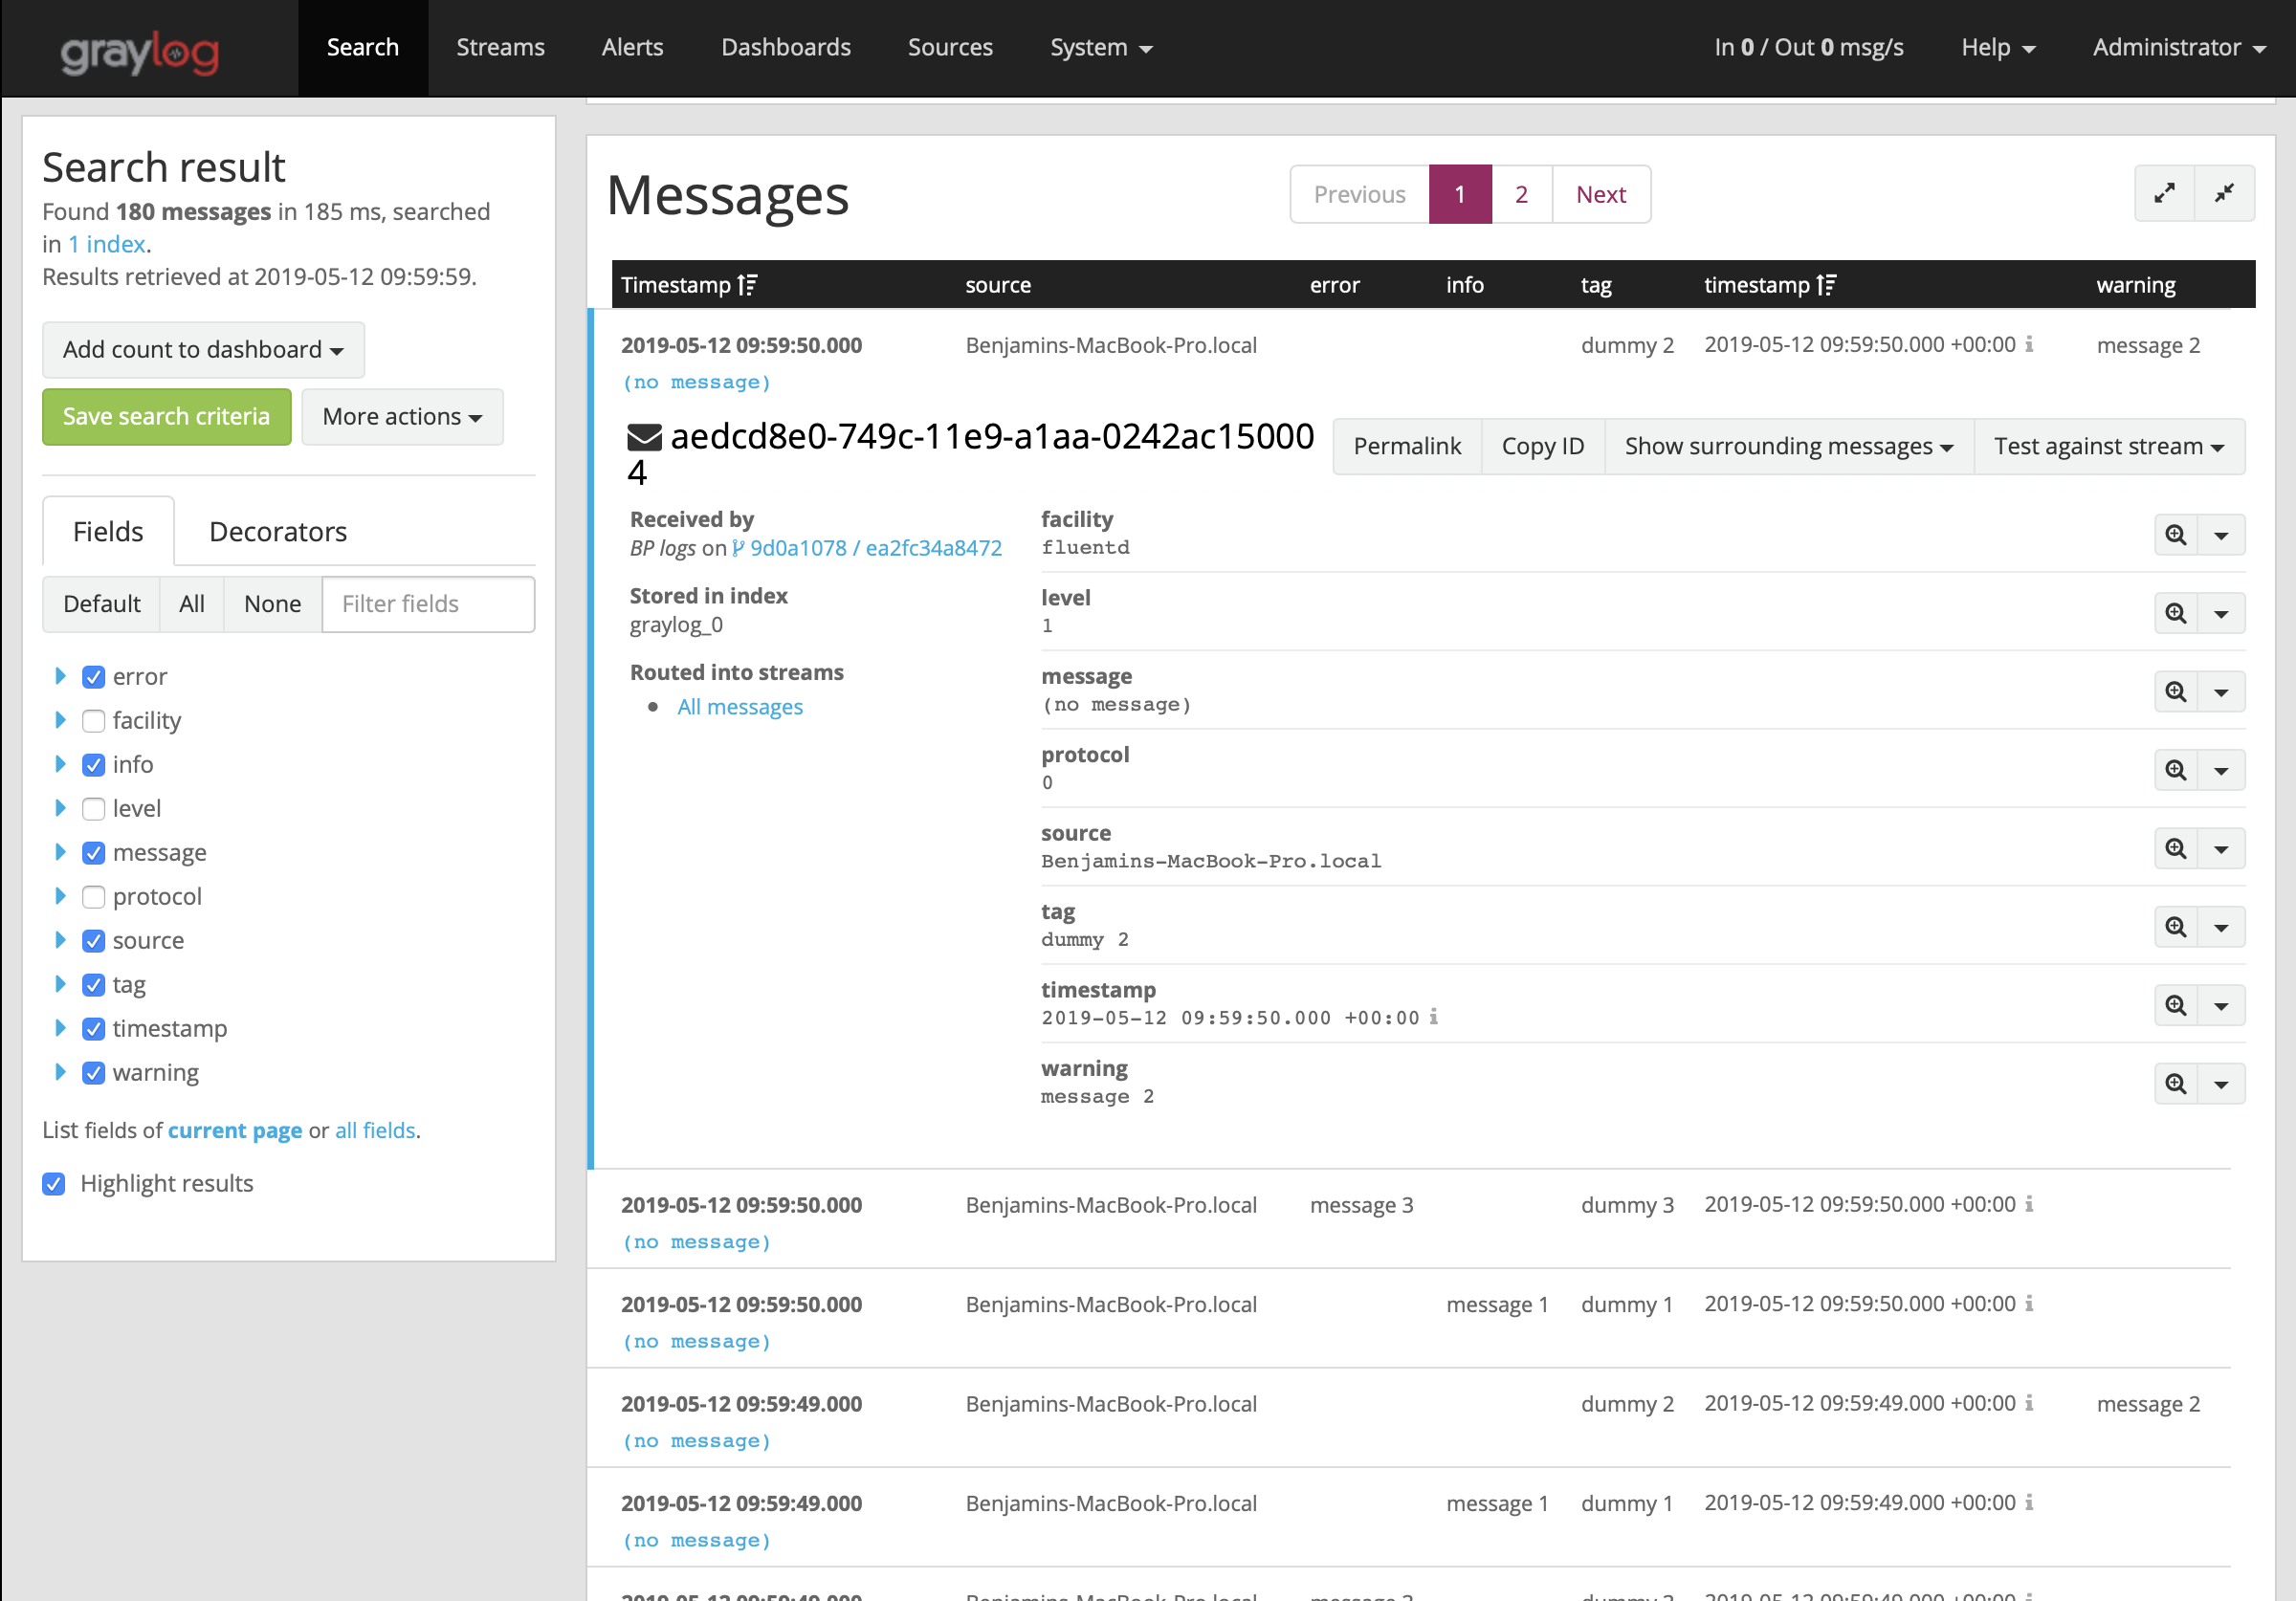
\includegraphics[scale=0.35]{img/graylog_detail}
    \caption[Graylog log detailscherm]{Graylog log detail}
\end{figure}

\begin{figure}[ht]
    \centering
    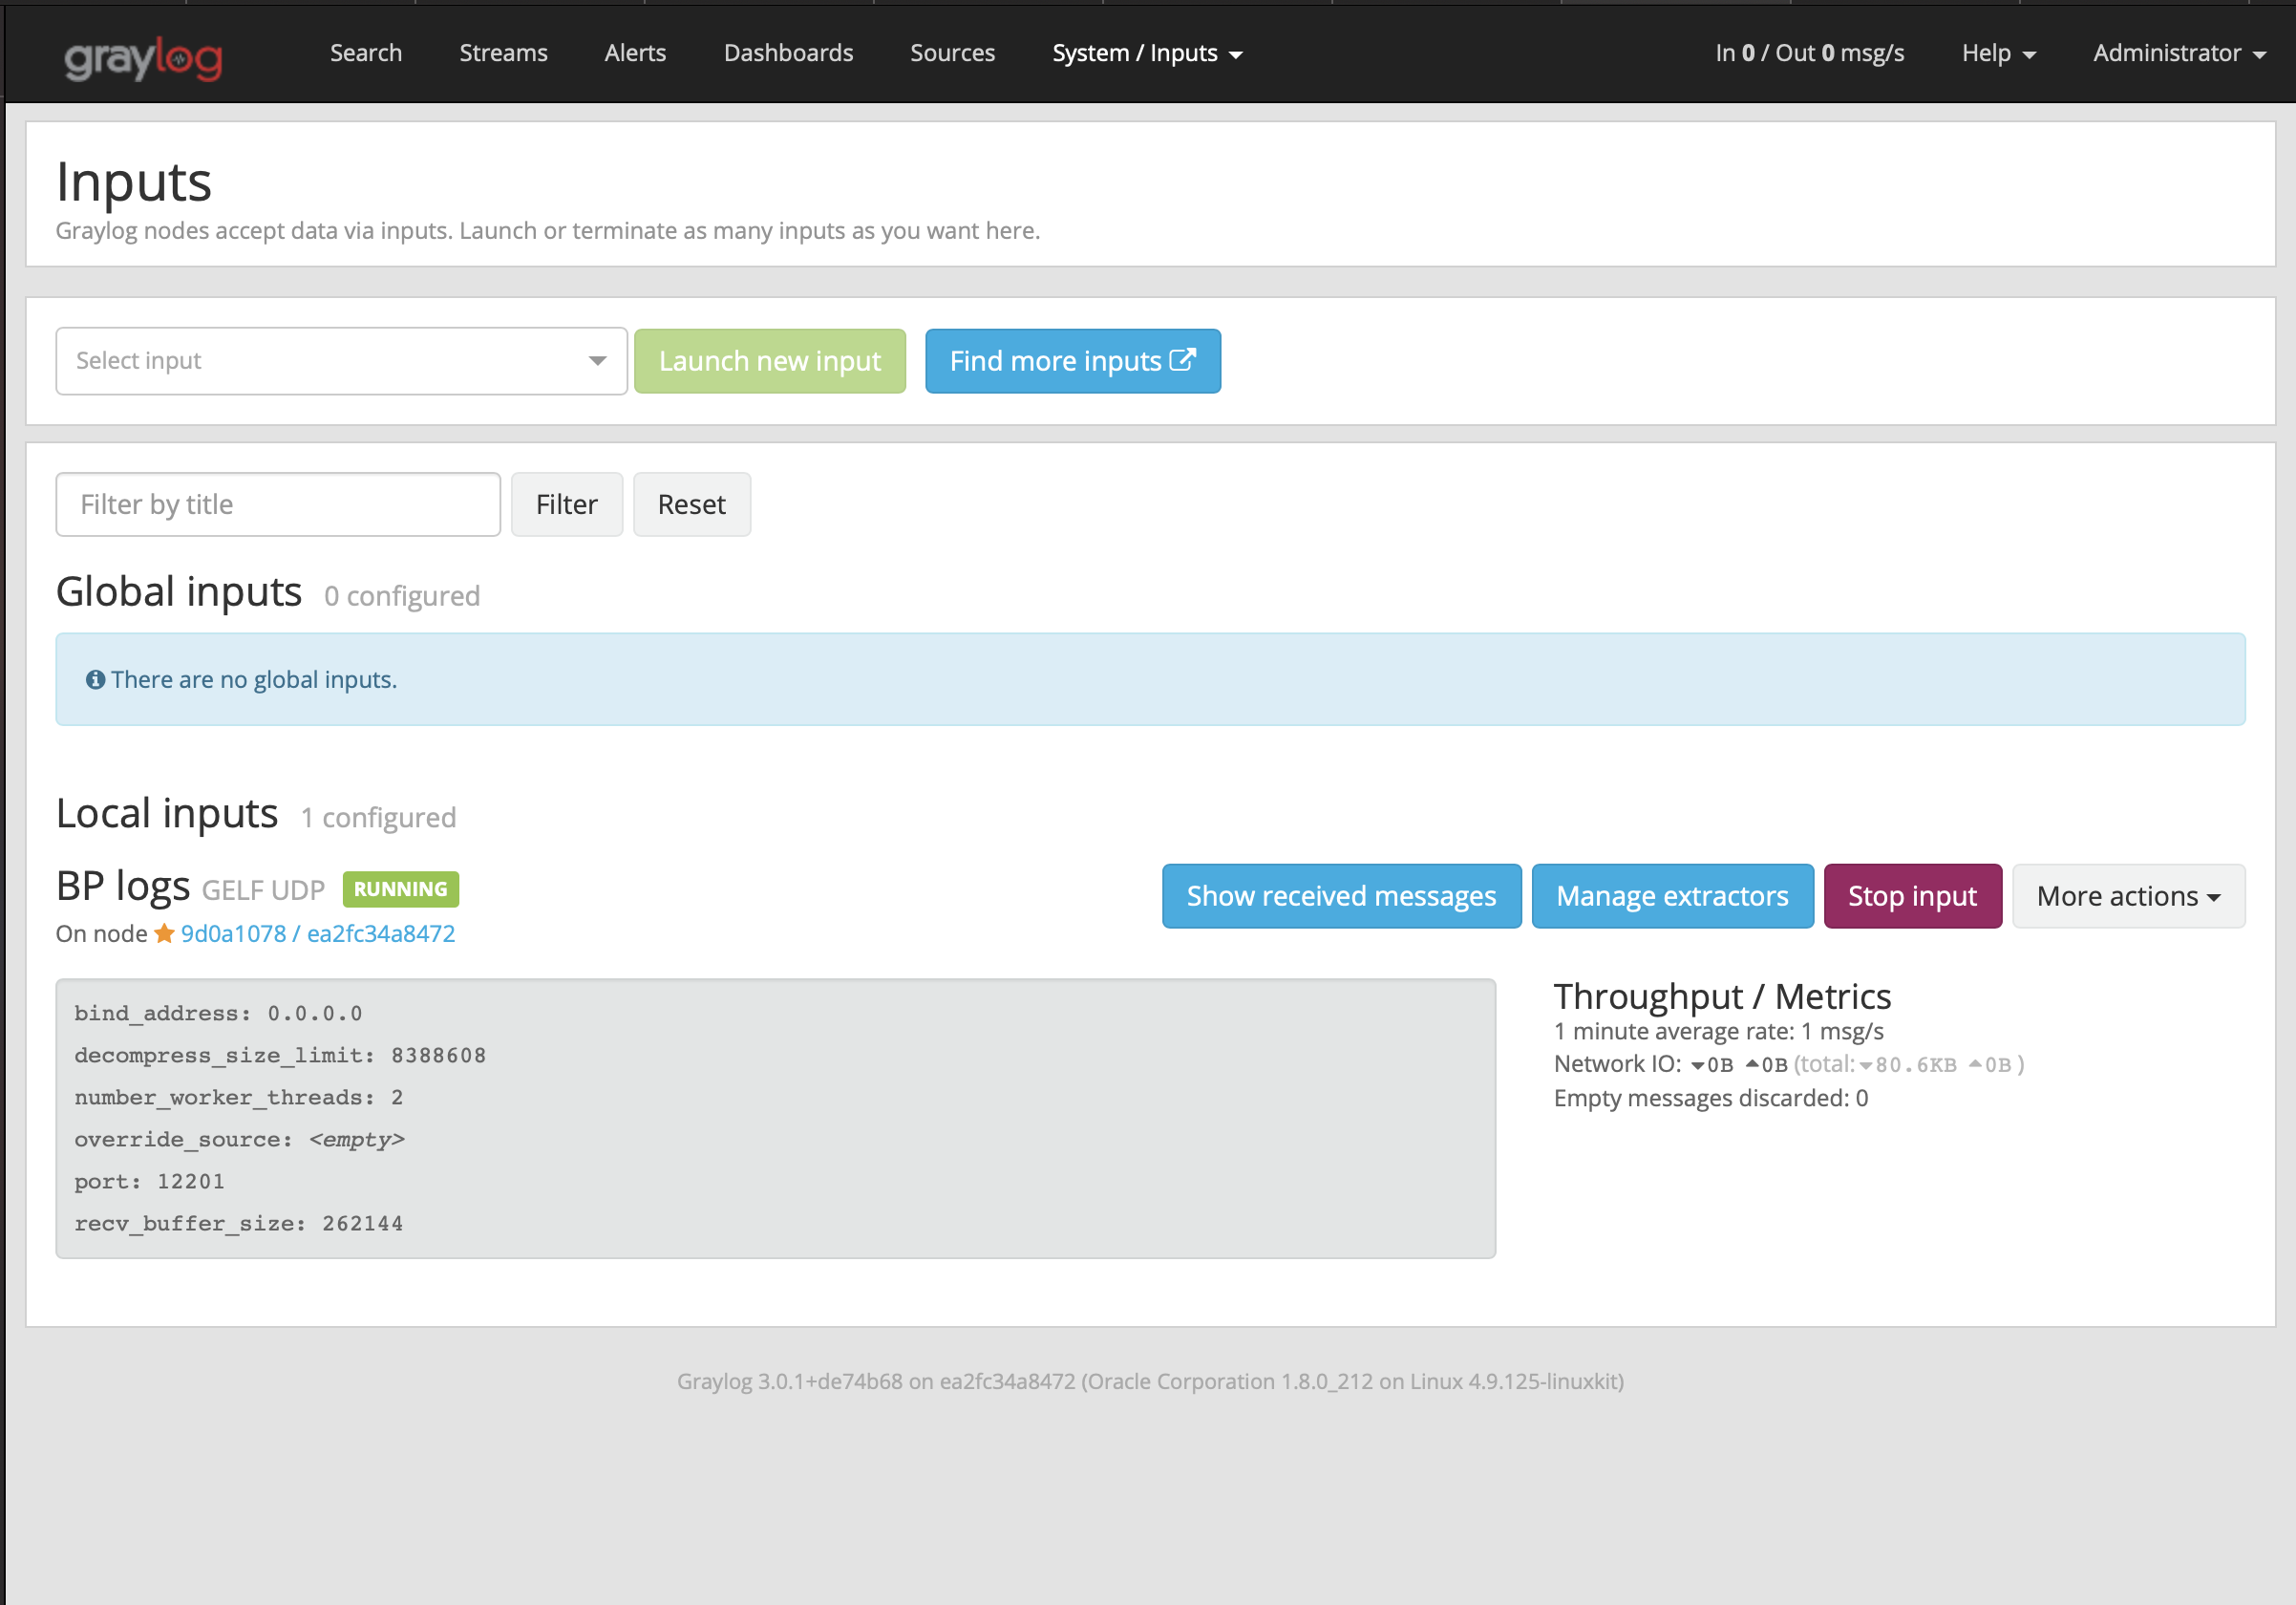
\includegraphics[scale=0.35]{img/graylog_input}
    \caption[Graylog input sherm]{Graylog input scherm}
\end{figure}

\subsection{Kubernetes omgeving}
Graylog configureren voor een Kubernetes omgeving is geen eenvoudige taak. Er wordt best gebruik gemaakt van github repositories om deze aan te passen naar eigen use case. Een dieper inzicht in deze complexe configuratie is overbodig in dit onderzoek en zal dus overgeslagen worden.

\section{Requirements}

\subsection{Must have}
\subsubsection{Moet open source zijn}
Voor elk van de onderzochte oplossingen geldt dezelfde score voor deze requirement, namelijk 5. Graylog is open source en kan vrij gebruikt worden op eigen servers.

\subsubsection{Ondersteuning voor cluster omgevingen zoals Kubernetes}
Zoals reeds vermeld in ~\ref{subsec:graylog} zorgt de ouderdom van deze oplossing ervoor dat deze niet geoptimaliseerd is voor een gedistribueerde omgeving. Graylog heeft wel al een oplossing aangeboden waardoor het mogelijk wordt om de oplossing in een Kubernetes cluster te plaatsen. 

Om deze reden krijgt Graylog een score van 2 op dit requirement.

\subsubsection{Moet een zo klein mogelijke impact hebben op de servers}
Voor Graylog geldt een zelfde uitleg als de ELK of Elastic stack voor dit requirement. Het maakt gebruik van Elasticsearch voor de opslag van logs. Het verschil hierin is dat Graylog gebruik maakt van een eigen log format GELF waardoor de opslag ervan geoptimaliseerd wordt \autocite{graylogdocs}.

Om deze reden krijgt Graylog een score van 3 op dit requirement.

\subsubsection{Moet kunnen scalen naargelang de groeiende Kubernetes cluster}
Het is mogelijk om Graylog mee te scalen met een groeiende cluster. Dit vergt echter wel de toevoeging van Fluentbit of Fluentd als een DaemonSet. Dit zorgt voor extra configuratie waar in een latere requirement rekening mee gehouden moet worden.

Om deze reden krijgt Graylog een score van 3 op dit requirement.

\subsection{Should have}
\subsubsection{Moet (relatief) eenvoudig te configureren zijn}
Zoals hierboven bij de requirement `Moet kunnen scalen naargelang de groeiende Kubernetes cluster`reeds vermeld werd, zorgt de toevoeging van Fluentbit of Fluentd voor extra configuratie. Dit komt bovenop de configuratie van Elasticsearch, Graylog zelf, en MongoDB voor het opslaan van de metadata. 
De configuratie van Elasticsearch is hetzelfde als reeds besproken in Hoofdstuk~\ref{ch:EFK} EFK. 

Om deze redenen krijgt Graylog een score van 2 op dit requirement.

\subsubsection{Moet (relatief) eenvoudig te gebruiken zijn}
Na de installatie is het moeilijkste achter de rug. De Graylog front end webservice beschikt over een soortgelijke functionaliteit als Kibana bij de ELK en EFK stacks. Bijgevolg kan een soortgelijk score gegeven worden aan Graylog, namelijk 4.

\subsubsection{Moet goed gedocumenteerd zijn}
De maturiteit van Graylog zorgt voor een overvloed aan documentatie voor het opstellen van Graylog in bijna elk soort omgeving, behalve Kubernetes. Aangezien de ondersteuning hiervoor nog steeds minimaal is, kan hetzelfde gezegd worden over de documentatie omtrent een Kubenernetes omgeving.

Omdat in het kader van dit onderzoek enkel gekeken wordt naar de documentatie omtrent Kubernetes deployment krijgt Graylog een score van 2 op dit requirement.

\subsubsection{Moet de logs overzichtelijk kunnen tonen}
De Graylog front end webservice beschikt over een soortgelijke functionaliteit als Kibana bij de ELK en EFK stacks. Hoewel de interface anders is opgebouwd dan die van Kibana kan dezelfde score gegeven worden aan elk van deze drie oplossingen, namelijk 5.

\subsubsection{Ondersteuning voor verschillende plugins die data extra kunnen verwerken of naar meerdere locaties kunnen doorsturen}
Dankzij de maturiteit van Graylog is er een grote hoeveelheid diverse plugins beschikbaar. Er is ook veel documentatie beschikbaar voor elke plugin en de manier waarop plugins in het algemeen gebruikt worden.

Om deze reden krijgt Graylog een score van 4 op dit requirement.

\subsubsection{Ondersteuning voor visualisatie zoals grafieken}
Voor Graylog geldt een zelfde uitleg als de ELK of Elastic stack voor dit requirement. Aangezien de de front end web service van Graylog en Kibana zo soortgelijk zijn, krijgen deze beiden dezelfde score, namelijk 5.

\subsection{Could have}
\subsubsection{Ondersteuning voor alerts}
Voor Graylog geldt een zelfde uitleg als de ELK of Elastic stack voor dit requirement. Aangezien de de front end web service van Graylog en Kibana zo soortgelijk zijn, krijgen deze beiden dezelfde score, namelijk 5.

\section{Resultaten}

Wanneer enkel gekeken wordt naar de eerste kolom met de scores op 5 is te zien dat Graylog slecht scoort op belangrijke requirements zoals ondersteuning voor cluster omgevingen, configuratie, en documentatie. De frontend van Graylog scoort dan weer goed met de overzichtelijkheid ervan. Wanneer de belangrijkheidsgraad in rekening wordt gebracht valt meteen op dat Graylog veel minder geschikt is voor de besproken use case dan de andere oplossingen. Een uitgebreide conclusie is te vinden in Hoofdstuk~\ref{ch:conclusie} Conclusie.

\begin{table}[]
    \begin{tabular}{| m{20em} | m{2cm} | m{2cm} | m{2cm} | }
        \hline
        \textbf{Requirement}                                                                                              & \textbf{Score (op 5)} & \textbf{Multiplier} & \textbf{Score met multiplier} \\ \hline
        Moet open source zijn                                                                                             & 5                     & 10                  & 50                            \\ \hline
        Ondersteuning voor cluster omgevingen zoals Kubernetes                                                            & 2                     & 10                  & 20                            \\ \hline
        Moet een zo klein mogelijke impact hebben op de servers                                                           & 3                     & 10                  & 30                            \\ \hline
        Moet kunnen scalen naargelang de groeiende Kubernetes cluster                                                     & 3                     & 10                  & 30                            \\ \hline
        Moet (relatief) eenvoudig te configureren zijn                                                                    & 2                     & 5                   & 10                            \\ \hline
        Moet (relatief) eenvoudig te gebruiken zijn                                                                       & 4                     & 5                   & 20                            \\ \hline
        Moet goed gedocumenteerd zijn                                                                                     & 2                     & 5                   & 10                            \\ \hline
        Moet de logs overzichtelijk kunnen tonen                                                                          & 5                     & 5                   & 25                            \\ \hline
        Ondersteuning voor verschillende plugins die data extra kunnen verwerken of naar meerdere locaties kan doorsturen & 4                     & 5                   & 20                            \\ \hline
        Ondersteuning voor visualisatie zoals grafieken                                                                   & 5                     & 5                   & 25                            \\ \hline
        Ondersteuning voor alerts                                                                                         & 5                     & 1                   & 5                             \\ \hline
        \textbf{Totale score}                                                                                             & 40                    &                     & 245                           \\ \hline
    \end{tabular}
    \caption{Graylog resultaten}
    \label{tab:graylog-resultaten}
\end{table}